

\section{Постановка задачи}

Нужно выделить информационные сущности продукта, описать их свойства и связи, распределить содержание по основным разделам и составить схему структуры. Работа описывает состав информации и ее вложенность.


AI Knowledge Agent превращает диалоги с ИИ в заметки для Obsidian. Студенты сохраняют материал для повторения, разработчики собирают технические объяснения и решения. Поэтому структура различает исходный диалог, извлеченные знания, план сохранения и фактический результат.


Описана текущая версия продукта. Она поддерживает импорт диалогов, анализ, создание заметок, дополнение существующих заметок, историю обработки и восстановление из резервных копий. При дополнении система добавляет разделы, теги и ссылки, сохраняя прежний текст заметки.


По умолчанию запись требует подтверждения пользователя. В настройках можно разрешить автоматическое выполнение небольших планов создания заметок, если они отвечают заданным правилам низкого риска. Решение о необходимости подтверждения принимает программа по установленным правилам.


\section{Основные разделы}

В продукте четыре основных раздела. Их названия совпадают с названиями текущего приложения. Остальные группы сведений вложены в них.


{\small\setlength{\tabcolsep}{5pt}\renewcommand{\arraystretch}{1.12}
\begin{longtable}{L{34mm}L{\dimexpr\textwidth-4\tabcolsep-34mm\relax}}
\caption{Основные разделы}\\
\toprule
\textbf{Раздел} & \textbf{Какая информация находится внутри} \\
\midrule\endfirsthead
\toprule
\textbf{Раздел} & \textbf{Какая информация находится внутри} \\
\midrule\endhead
\bottomrule\endfoot
Рабочая область & Сведения об импортированном диалоге, ход обработки, темы и извлеченные знания, план сохранения, причины согласования и фактический результат. \\[6pt]
История & Список обработок с датами и состояниями, доступ к их подробностям и изменениям, резервные копии и результат восстановления. \\[6pt]
Граф знаний & Сохраненные заметки как узлы графа: название, путь и теги. Связи между заметками, соседние материалы, вид связи и признак неоднозначности. \\[6pt]
Настройки & База знаний, хранилище данных, основная модель ИИ и модель семантического поиска, правила сохранения, параметры длинного текста и повторного планирования. \\[6pt]
\end{longtable}}

\textbf{Рабочая область} объединяет исходный диалог, анализ, план и результат записи. Импорт принимает вставленный текст, данные из буфера обмена, Markdown, TXT, экспорт ChatGPT и Claude в JSON, а также HTML с текстом разговора. Разные источники приводятся к общей структуре диалога.


\textbf{История} позволяет найти прошлую обработку по названию разговора, дате и состоянию. Ее подробности относятся к тому же объекту обработки, который используется в рабочей области.


\textbf{Граф знаний} строится по существующим WikiLink и полю related в заметках. Он показывает реальные связи, включая неоднозначные соответствия названий. В графе доступны название, путь, теги и соседние заметки. Полный текст хранится в файлах Obsidian.


\textbf{Настройки} содержат параметры подключения и правила работы с данными. Ключи доступа не возвращаются вместе с общими сведениями: приложение сообщает только, настроен ли ключ. Названия четырех разделов содержат не более двух слов.


\clearpage
\section{Информационные сущности}

Выделены двенадцать сущностей. Они описывают информацию продукта. События обработки, решение о согласовании и результаты проверок входят в сведения соответствующих сущностей.


\subsection{Исходный материал и анализ}

{\small\setlength{\tabcolsep}{5pt}\renewcommand{\arraystretch}{1.12}
\begin{longtable}{L{34mm}L{\dimexpr\textwidth-4\tabcolsep-34mm\relax}}
\caption{Исходный материал и анализ}\\
\toprule
\textbf{Сущность} & \textbf{Какие сведения содержит} \\
\midrule\endfirsthead
\toprule
\textbf{Сущность} & \textbf{Какие сведения содержит} \\
\midrule\endhead
\bottomrule\endfoot
Диалог & Идентификатор, название, источник, дата импорта, сообщения и признак совпадения содержания для обнаружения повторного импорта. \\[6pt]
Сообщение & Принадлежность диалогу, порядок, роль участника, текст и время, если оно есть в исходном материале. Неизвестная роль сохраняется явно. \\[6pt]
Обработка & Идентификатор, исходный диалог, время начала и завершения, состояние, текущий этап, ошибка, события и расход токенов. С ней связаны анализ, план и результат. \\[6pt]
Тема & Идентификатор внутри анализа, название, краткое описание, диапазон сообщений и уверенность определения темы. \\[6pt]
Извлеченное знание & Идентификатор, тема, название, краткое содержание, основные положения, тип, оценка уверенности и предложение о форме сохранения. При наличии указаны исходные цитаты, вопрос пользователя, его понимание или заблуждение, объяснение ИИ и найденные похожие заметки. \\[6pt]
\end{longtable}}

Один диалог можно обработать несколько раз. Поэтому состояние и результаты принадлежат обработке. Извлеченное знание еще не считается сохраненной заметкой.


Тип знания принимает одно из шести значений: понятие, алгоритм, фреймворк, технология, вопрос или учебная заметка. Для формы сохранения предусмотрены отдельная заметка, раздел другой заметки и пропуск.


\clearpage
\subsection{План, материалы и результат}

{\small\setlength{\tabcolsep}{5pt}\renewcommand{\arraystretch}{1.12}
\begin{longtable}{L{34mm}L{\dimexpr\textwidth-4\tabcolsep-34mm\relax}}
\caption{План, материалы и результат}\\
\toprule
\textbf{Сущность} & \textbf{Какие сведения содержит} \\
\midrule\endfirsthead
\toprule
\textbf{Сущность} & \textbf{Какие сведения содержит} \\
\midrule\endhead
\bottomrule\endfoot
План сохранения & Принадлежность обработке, действия, общее обоснование, затрагиваемые файлы и счетчик повторного планирования. Решение о согласовании содержит уровень риска, причины, показатели и требование подтверждения. \\[6pt]
Действие плана & Вид: создание, дополнение, пропуск или отметка конфликта. В зависимости от вида указаны исходные знания, целевой файл, разделы, теги, ссылки и причина. Для конфликта сохраняются спорные сведения. Пользователь может исключить предложенные изменения из выполнения. \\[6pt]
Заметка & Путь как идентификатор, название, полный текст и разделы, теги и альтернативные названия. Тип, источник и даты берутся из метаданных при их наличии. Для графа используются название, путь и теги. \\[6pt]
Связь заметок & Исходная и целевая заметки, вид связи WikiLink или related, название цели и признак неоднозначного соответствия. Граф использует связи между существующими заметками. \\[6pt]
Отчет обработки & Итоговое состояние, созданные и дополненные заметки, ошибки выполнения, результаты проверки файлов, изменения и сведения об откате при неудачной записи. Пропуски и конфликты доступны в связанном плане. \\[6pt]
Резервная копия & Место хранения, исходный файл, метка связанной операции, дата, размер и содержимое файла перед изменением. При восстановлении указан целевой файл; перед заменой сохраняется его текущая версия. \\[6pt]
Настройки & Пути к базе знаний, новым заметкам, резервным копиям и данным SQLite; параметры основной модели и Embedding, состояние подключения, правила согласования, размеры частей длинного текста и предел повторного планирования. \\[6pt]
\end{longtable}}

Создание, дополнение, пропуск и отметка конфликта уже входят в текущую версию. Дополнение сохраняет прежний текст и добавляет новые разделы, теги или ссылки. Перед изменением существующего файла создается резервная копия.


План сообщает, что предполагается сделать. Отчет содержит фактический результат. Восстановление из копии доступно в истории. Для настроек хранилища различаются текущий путь и сохраненный путь, который начнет действовать после перезапуска.


\clearpage
\section{Связи и вложенность}

Обозначение 1:N означает связь одного объекта с несколькими. Число 0 указывает, что связанный объект может отсутствовать, например до окончания обработки.


{\small\setlength{\tabcolsep}{5pt}\renewcommand{\arraystretch}{1.12}
\begin{longtable}{L{42mm}L{23mm}L{\dimexpr\textwidth-6\tabcolsep-65mm\relax}}
\caption{Связи и вложенность}\\
\toprule
\textbf{Объекты} & \textbf{Количество} & \textbf{Смысл связи} \\
\midrule\endfirsthead
\toprule
\textbf{Объекты} & \textbf{Количество} & \textbf{Смысл связи} \\
\midrule\endhead
\bottomrule\endfoot
Диалог и сообщения & 1:1..N & Сообщения вложены в диалог и имеют порядок. \\[6pt]
Диалог и обработки & 1:0..N & У одного исходного разговора может быть несколько попыток обработки. \\[6pt]
Обработка и темы & 1:0..N & Темы выделены в конкретном анализе и связаны с исходными сообщениями. \\[6pt]
Обработка и знания & 1:0..N & Каждое извлеченное знание связано с одной темой конкретной обработки. \\[6pt]
Обработка и план & 1:0..1 & У обработки есть текущий план. При повторном планировании растет его счетчик. \\[6pt]
План и действия & 1:0..N & Действия вложены в план. Пустой результат анализа может не требовать записи. \\[6pt]
Действие и заметка & 1:0..1 & Создание или дополнение относится к одному целевому файлу. Пропуск не создает заметку. \\[6pt]
Знания и заметки & N:M & Одна заметка может объединять несколько извлеченных знаний. Связь с исходными знаниями сохраняется в действиях плана. \\[6pt]
Заметки между собой & N:M & Заметки связаны ссылками и остаются отдельными материалами. Эта связь образует ребра графа. \\[6pt]
Обработка и отчет & 1:0..1 & Результат относится к одной обработке. До выполнения отчет может отсутствовать. \\[6pt]
Обработка и копии & 1:0..N & При дополнении файлов обработка получает резервные копии. Создание нового файла не требует копии прежней версии. \\[6pt]
\end{longtable}}

Диалог содержит сообщения. План содержит действия. Заметка содержит собственные разделы текста. Например, Attention может быть отдельной заметкой, а Self-Attention может быть разделом внутри нее. Это отношения вложенности.


Ссылка между двумя заметками описывает связь отдельных объектов. Граф представляет сохраненные заметки и их реальные ссылки. Он не создает новые смысловые отношения между материалами.


История и рабочая область дают доступ к одной обработке по ее идентификатору. План, анализ и результат не копируются в отдельные объекты для каждого раздела.


Приложение предназначено для одного локального пользователя. Учетные записи и роли доступа в структуру не включены. Полные тексты заметок остаются в Obsidian; отдельного редактора всей библиотеки внутри приложения нет.


\clearpage
\section{Схема структуры}

Схема показывает разделы и вложенные группы информации. Каждый блок описывает содержание соответствующего раздела.


\begin{figure}[H]\centering
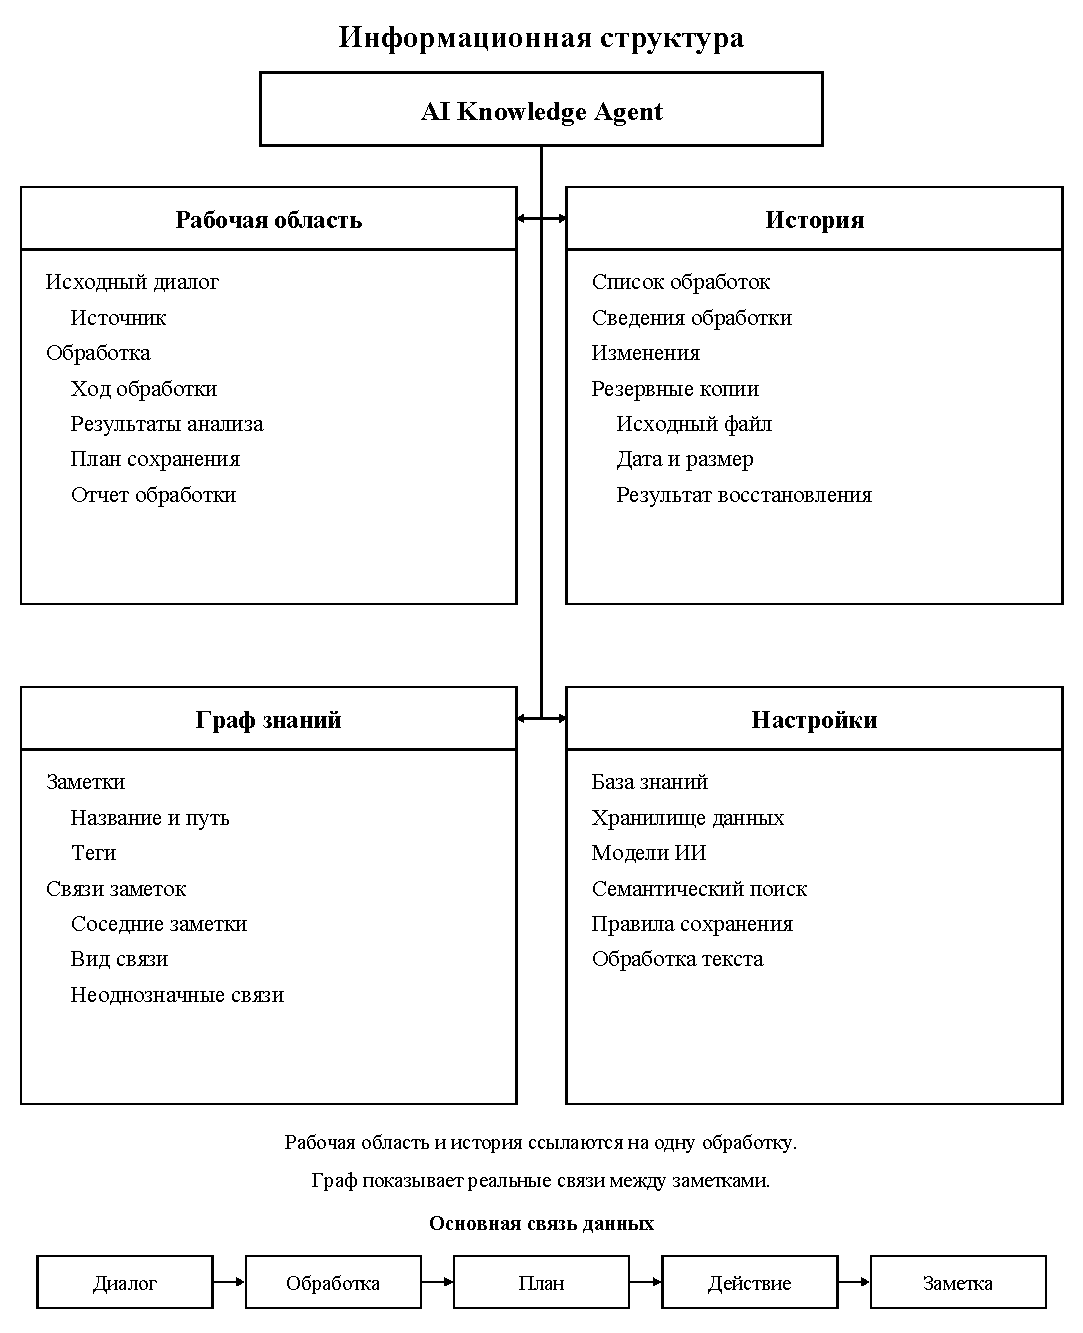
\includegraphics[width=\textwidth]{figures/information-architecture.pdf}
\caption{Разделы и вложенные группы сведений}
\end{figure}

\clearpage
\subsection{Текстовая структура}

{\fontsize{9}{10.7}\selectfont\begin{verbatim}
AI Knowledge Agent
+-- Рабочая область
|   +-- Исходный диалог
|   |   +-- Источник
|   +-- Обработка
|       +-- Ход обработки
|       +-- Результаты анализа
|       +-- План сохранения
|       +-- Отчет обработки
+-- История
|   +-- Список обработок
|   +-- Сведения обработки
|   +-- Изменения
|   +-- Резервные копии
|       +-- Исходный файл
|       +-- Дата и размер
|       +-- Результат восстановления
+-- Граф знаний
|   +-- Заметки
|   |   +-- Название и путь
|   |   +-- Теги
|   +-- Связи заметок
|       +-- Соседние заметки
|       +-- Вид связи
|       +-- Неоднозначные связи
+-- Настройки
    +-- База знаний
    +-- Хранилище данных
    +-- Модели ИИ
    +-- Семантический поиск
    +-- Правила сохранения
    +-- Обработка текста
\end{verbatim}}

Результаты анализа содержат темы, знания, их типы и найденные похожие заметки. План содержит действия и сведения о согласовании. Отчет объединяет результат записи, проверку, изменения и возможный откат.


История позволяет вернуться к той же обработке и найти резервные копии. Граф дает другой способ изучить сохраненные материалы через их связи.


\section{Заключение}

Составлена информационная архитектура текущей версии продукта: четыре основных раздела и двенадцать сущностей. Для сущностей описаны свойства, связи и вложенность. Структура охватывает импорт, анализ, создание и дополнение заметок, историю, восстановление, граф знаний и настройки.


